\documentclass[letterpaper]{article}
\usepackage{aaai19}
\usepackage{times} 
\usepackage{helvet}
\usepackage{courier} 
\usepackage[hyphens]{url}
\usepackage{graphicx}
\urlstyle{rm}
\def\UrlFont{\rm}
\usepackage{graphicx}
\frenchspacing
\setlength{\pdfpagewidth}{8.5in}
\setlength{\pdfpageheight}{11in}
% custom packages%
\usepackage{amsmath}
\usepackage{enumitem}
\usepackage{subcaption}


\pdfinfo{
/Title (Measuring the Influence of Twitter Bots during the 2018 US Midterm Election)
/Author ()
}

\setcounter{secnumdepth}{2} %May be changed to 1 or 2 if section numbers are desired.

\title{Measuring the Influence of Twitter Bots during the 2018 US Midterm Election}

\begin{document}

\maketitle

\begin{abstract}
    Use of bots in social media and its consequences has been a subject of great public interest. In this study, we measure the influence of bots during 
    the 2018 US Midterm Elections. Between October 31, 2018 and November 7, 2018 we collected 6.48M tweets and 1.6M profile data from Twitter. We used 
    Machine Learning techniques to separate bot and human accounts and found that 1\% of the
    top bots influenced the creation of 11\% of all the tweets. Additionally, for URLs which were retweeted more than ten times in our dataset, we found that the 
    total influence percentage of bots was double their size. 
    Influence is a number we give to a tweet which measures 
    the expected number of time the tweet gets retweeted over all possible diffusion scenarios. Influence is converted to percentage by using the sum of user wise influence 
    throughout the dataset.
\end{abstract}

\section{Introduction}
\label{sec:introduction}

Twitter is a social media where short messages get exchanged. Messages shared by a user are shown to
their followers and to followers of those who share the message. These messages are called Tweets. Sharing can be done by retweeting
(sharing) or replying to the tweet. When Alice replies/retweets, a tweet made by Bob, Alice and Bob's followers will see the tweet. In this
way, messages spread. Having massive followers, getting many retweets, getting retweeted by people with massive followers or advertising can make a tweet viral.\par

People use social media, at least in part, to form an opinion about lifestyle, health, politics, and purchase \cite{varol2017early}. 
Due to the power of social media in influencing opinion, various ethical and unethical techniques have been devised to reach a big audience. 
One such unethical technique is the use of bots. Social bots are account controlled wholly or partially by a computer algorithm. 
These bots can generate content and interact with human users often imitating humans \cite{ferrara2016rise}.
A US special counsel investigation found that Twitter accounts of US personas were being operated as a botnet (a network of bots) to amplify content. 
During the 2016 US Presidential Election, they chose candidates to support and oppose \cite{luceri2019red,mueller_investigation}. 
These propaganda bots were found to be high volume, multichannel, rapid, continuous, repetitive, inaccurate, and inconsistent \cite{paul2016russian}. \par

Past studies have explored the political polarization \cite{munger2017don,rizoiu2018debatenight,gruzd2014investigating,bovet2019influence}, origin of bots 
\cite{zannettou2019let,zannettou2019characterizing} and the spread of fake news \cite{vosoughi2018spread,shao2018spread,lazer2018science,bovet2019influence,grinberg2019fake}
on twitter. Previous US Election has been studied before. Most studies focus on 2016 Election \cite{bovet2019influence,rizoiu2018debatenight,bessi2016social,howard2018algorithms,howard2016bots}. \cite{deb2019perils} 
studied the 2018 Midterm Election.\par 

Few studies perform a large scale quantitative study of the role played by bots during a significant event. To fill the gaps in the literature, 
we measured the influence of bots during the 2018 US Midterm Election. \par


\subsection{Summary and Findings}

\begin{itemize}
    \item 10.5\% of the users in the datasets were bots. They made 12.6\% of the tweets and created 22\% of the total influence.
    \item On Average, bots were twice as influential as humans
    \item Top 1\% of the bots influenced the creation of 11\% of all the retweets during this time.
    \item In average a single URL was shared 27.84 times in 1.97 cascades. URL cascade is formed when a Tweet mentions a URL. Any further retweet belong to the same cascade.
    \item For URLs which were shared more than ten times, the influence percentage of bots was double their size.
    \item 81.64\% of all interaction (retweets and replies) took place between humans, and 2.87\% took place between bots. 6.37\% was bot-human, and 9.14\% was human-bot interaction.
    \item Most of the codes and notebooks are shared publicly in https://github.com/warproxxx/2018Midterm to help future researchers and ensures transparency.
\end{itemize}

*
\section{Related Work}
\label{sec:related}

\subsection{Social Media and Bots}
People are spending more and more time on social media. Globally, people spend 2 hours and 23 minutes on average in Social Media. 40\%  people use social media to stay up to date 
with news and current events \cite{2019_social_flagship_report}. 68\% of American adults get their news from
social media while 42\% find news on social media to be mostly accurate \cite{pew_research_news}.\par

Twitter is not the most popular social media. 12\% of US adults get news from Twitter compared to Facebook's 43\% \cite{pew_research_news}. However, 
Twitter is the number one platform for government leaders. 97\% of all UN members have an official presence in Twitter \cite{twiplomacy}. Furthermore, Twitter API provides easy access to data.
Consequently, Twitter has been widely studied \cite{rizoiu2018debatenight,grinberg2019fake,bovet2019influence,morstatter2018alt,munger2017don,gruzd2014investigating,zannettou2019characterizing,howard2016bots}.
\par

Social Media have been used for positives like democratizing online discussion, organizing civil movements \cite{gonzalez2013broadcasters}, augumenting public health 
\cite{dredze2012social}, forecasting \cite{asur2010predicting,nguyen2015sentiment,liu2016predicting}, forming social connections \cite{ellison2007benefits}, and 
for other greater goods \cite{moorhead2013new,househ2014empowering}. However, recently, more focus is being put on the negatives with high focus on disinformation and bots
\cite{forelle2015political,bradshaw2017troops,marwick2017media}. \par

Different types of bots exist in social media. A simple bot will post predetermined messages at predetermined intervals \cite{haustein2016tweets}. Bots are also used to increase followers
and make an account appear popular \cite{cresci2015fame}. Botnets are a network of bots working together. The word Botnet is also used to refers to a network of compromised computer. However, in this report, 
the word botnet refers to a network of social media bots working together to make an influence and should not be confused with the other definition. Many botnets use a hybrid human/automation 
approach \cite{grimme2018changing}. Botnets have been used to promote spam \cite{ferrara2018measuring}, which seem to shifted to social media due to the effectiveness of spam filter \cite{gao2010detecting,chu2012detecting,ferrara2018measuring}, 
manipulate stocks \cite{ferrara2015manipulation}, manipulate elections \cite{morstatter2018alt}, 
and for various other purposes \cite{abokhodair2015dissecting}.
Botnets were detected as early as 2010 US Midterm Election \cite{mitter2014categorization}. Over time, their use and study have increased. 
Studies have detected and analyzed bots in the 2017 German Federal Election \cite{morstatter2018alt} ,2017 French Presidential Election \cite{ferrara2017disinformation} and during 
various US Elections \cite{mitter2014categorization,bovet2019influence,rizoiu2018debatenight,bessi2016social,howard2018algorithms,howard2016bots,deb2019perils}. In Elections, 
they have been used to support candidates \cite{luceri2019red}, attack people \cite{mueller_investigation} and spread fake news \cite{vosoughi2018spread,grinberg2019fake}. 
Political bots are active beyond the election time. \cite{stewart2018examining} found that Russian bots infiltrated both right and left-leaning communities and spread different narratives 
\cite{mueller_investigation}. \par

In Twitter, bots share content 
in multiple channel \cite{paul2016russian}. This activity is in line with literature which shows that information from multiple sources appears more trustworthy than a single one \cite{harkins1981multiple}. 
 Bots attack people. Attacking trustworthiness has been shown to diminish the credibility of the Original Poster \cite{pornpitakpan2004persuasiveness}. 
Bots are continuous, repetitive, but most of the times, they are also far from reality \cite{paul2016russian}. The high volume seems to ensure early exposure and \cite{petty1994think} shows that early
 first impression is more likely to be accepted by the brain. Due to a phenomenon called Sleeper Effect, where information gets disassociated from the source while remembering \cite{underwood1998memory,paul2016russian}
 low credibility sources can have persuasive power to unbiased or neutral people. As a boost to sleeper effect, people are 31\% more likely to remember what they see on twitter, 
 compared to the normal web \cite{twitter_remember}. \par

\subsection{Bot Detection}
Most studies \cite{rizoiu2018debatenight,yang2019arming,shao2018spread} use Botometer\cite{davis2016botornot,yang2019arming} for bot detection.
Botometer's Machine Learning algorithm provides an account-level bot classification. Botometer classifies account partially and completely automatized as bots. 
Botometer has some false positives. Its detection of organizational accounts as bots have been highly criticized \cite{varol2017early} \cite{botometer_tweet}. However, even with its false positive, 
Botometer has no transparent competitor and 
remains the most accurate bot detection system in academia. \par

Botometer uses more than a thousand features created from temporal activity, network structure, content analysis, sentiment analysis, and user profile data to
determine a bot score \cite{davis2016botornot,yang2019arming}. \cite{bessi2016social} illustrated that profile customization, geographical metadata, and activity statistics provided the strongest signals for bot detection. \cite{ferrara2017disinformation} and \cite{kudugunta2018deep} used various machine learning techniques on these features. \cite{ferrara2017disinformation}
obtained 93\% accuracy with an AUC-ROC score of 92\% in their best model using Random Forest classifier. \cite{kudugunta2018deep} used 3,000 labeled examples to train a system with an AUC greater than 99\%
using Adaboost Classifier with Over Sampling and Undersampling of data using the SMOTENN algorithm. \cite{kudugunta2018deep} also presented a tweet level classification using contextual LSTM
classifier with tweet metadata and deep learning. \par


Most studies show that 10-20\% in social media are bots. In earlier studies, the number was on the higher side. 18\% of users in \cite{bovet2019influence}'s study were bots.
A more recent study by \cite{deb2019perils} states that their number may have dropped.

\subsection{Influence Detection}
\cite{zannettou2019let} uses Hawkes Process to determine the influence Iranian and Russian bots had on pushing URLs in 4 social media platforms. They found that Russian trolls were extraordinarily 
influential and efficient in spreading URLs. \cite{shao2018spread} found that bots amplify URLs in early moments before an article goes viral, while \cite{ferrara2018measuring} 
found the same for spam. Bots target users with many followers through replies and manipulation. This method was very efficient. \par


\cite{shao2018spread} also found that articles spread 
mostly through tweets and retweets and much lesser from replies. Their study showed that people do not discriminate between resources shared by humans and bots. 
\cite{shao2018spread} and \cite{grinberg2019fake} found super spreaders. Moreover,  \cite{grinberg2019fake} found that  1\% of individuals accounted for 80\% of fake news exposure. 
\cite{varol2017early} also found that 2\% user accounts were responsible for 60\% of the conversation. \par

\cite{rizoiu2018debatenight} found that social bots were 2.5 times more influential than humans. They introduce a scalable algorithm for estimating user influence in retweet cascades. 
For each tweet in an information cascade, it uses time of post and the number of followers to determine the probability of whether a tweet is a retweet of another. They then find influence which can be used 
to find out how many users the tweet possibly influenced to retweet. It was tested successfully in artificial social media. Other studies have attempted to measure influence before this. 
\cite{weng2010twitterrank} used eigenvector centrality of the connection to measure influence, but it is not scalable into big cascades. There are other methods like 
\cite{rodriguez2011uncovering,cho2013latent,linderman2014discovering} but they either have scaling issue or require full diffusion graph, which Twitter does not provide.

\section{Methods}
\label{sec:method}
\subsection{Data Collection}
Twenty-nine manually identified keywords, and names of all 53 House candidates and 27 Senate candidates were used to collect live data from Twitter. The manually defined keywords are in 
Table \ref{tab:manual-keywords}

\begin{table}[]
    \centering
    \begin{tabular}{ll}
    • 2018Midterms & • resist \\
    • 2018MidtermElections & • VOTE \\
    • Election2018 & • GAEarlyVoting \\
    • ElectionDay & • EarlyVoting \\
    • MAGA2018 & • plus1 \\
    • MAGA & • IVoted \\
    • Trump2020 & • WinBlue \\
    • AmericaFirst & • WinRed \\
    • TheResistance & • BlueWave \\
    • WalkAwayFromRepublicans2018 & • RedWave \\
    • VoteThemOut & • republican2018 \\
    • 2018Senate & • democrat2018 \\
    • VoteRed & • Republican \\
    • Voteblue & • Democrat \\
    • WalkAwayFromDemocrats2018 & 
    \end{tabular}
    \caption{Manual Keywords}
    \label{tab:manual-keywords}
\end{table}

Twitter provides Streaming API, Search API, and a premium Firehose API to provide access to tweets. Streaming API provides limited access to live data (thus also called 1\% API)
 while Firehose API
provides complete data. However, due to the associated costs, Firehose API was not an option in this study. \cite{morstatter2013sample} compares the Streaming API with Firehose API.
They found that Streaming API was nearly as good as a random sample of Firehose API when the dataset was large enough. Although the 1\% API was not as good as a 1\% random sample from the Firehose API in 
all of their tests, it estimated the top hashtags correctly when the data was large enough. It recommended the creation of specific parameters and using a large sample. 
Due to the possible issues in Streaming API, \cite{bessi2016social} recommends using Twitter Search API. 

\par In this study, we use Streaming API with many keywords as suggested by \cite{morstatter2013sample} to collect a large dataset. While collecting data, information about the tweeter and the tweet was collected. 

We collected following information about a tweet:
\begin{enumerate}[label=\textbf{\arabic*}]
    \item \textbf{Timestamp:} UTC Timestamp in which the post was made
    \item \textbf{ID:} Post ID provided by twitter
    \item \textbf{Text:} Text in the tweet and the parent tweet if the tweet is a reply
    \item \textbf{User:} Username of the tweeter/retweeter/replier
    \item \textbf{Replies:} The number of replies the tweet has received. During live collection, this value is zero. We collect them during recollection of top tweets.
    \item \textbf{Retweets:} The number of retweets the tweet has received. During live collection, this value is zero. We collect them during recollection of top tweets.
    \item \textbf{Likes:} The number of likes the tweet has received. During live collection, this value is zero. We collect them during recollection of top tweets.
    \item \textbf{Reply To ID:} The ID of the parents tweet if this is retweet or a reply.
    \item \textbf{Response Type:} Either Tweet or Retweet or Reply
\end{enumerate}
\bigskip

We collected the following profile information from the Twitter API:
\begin{enumerate}[label=\textbf{\arabic*}]
    \item \textbf{Username:} Username of the user who posted the tweet
    \item \textbf{Location:} Binary if geolocation is enabled
    \item \textbf{Is Verified:} A binary if the profile has been verified
    \item \textbf{Total Tweets:} Total number of tweets created by the user
    \item \textbf{Total Following:} Total accounts the user is following
    \item \textbf{Total Followers:} Total Followers
    \item \textbf{Total Listed:} Number of times a user has been listed
    \item \textbf{Total Status:} Total Status
    \item \textbf{Total Likes:} Total likes the user has received
    \item \textbf{Has Background:}  Binary if an account has a background
    \item \textbf{Is Protected:}  Binary if an account is protected
    \item \textbf{Profile Modified:}  Binary if a profile has been modified
\end{enumerate}
\bigskip
\cite{kudugunta2018deep} and \cite{ferrara2017disinformation} use the same parameters in their machine learning architecture. \par

We collected Tweets from October 31, 2018 (1 AM UTC) to November 7, 2018 (midnight UTC). On July 18, 2019, we used Twitter API to rescrape the top 100k most retweeted which did not 
exist in our dataset.

\subsection{Data Processing}
First, we manually removed irrelevant tweets. We created keywords find and remove these irrelevant data.\par

We used SentiStrength and VADER Sentiment analysis in the Tweets. SentiStrength \cite{thelwall2010sentiment} is used to annotate short, informal tweet like texts \cite{bessi2016social}. 
It can capture positive and negative emotions at an accuracy of 60.6\% and 72.8\%. SentiStrength gives a positive and negative score between 0 and 4. The positive sentiment is subtracted 
from the negative like in \cite{bessi2016social} to get a whole number. VADER is a rule-based sentiment classification designed for use in social media data. VADER was found to outperform 
individual human raters with an F1 accuracy of 0.96 compared to 0.84 for humans \cite{hutto2014vader}.

\subsection{Bot Detection}
Detecting bots on the wild is more complicated than against a validation set \cite{bovet2019influence,varol2017early,ferrara2016rise}. The collected dataset had 1.7M 
users. Although Botometer is publicly available, getting information for 1.7M data would be expensive. So the following steps were used to train a bot detection system:

\begin{itemize}
    \item \cite{cresci2017paradigm} provided a labeled account level bot or not data with relevant features that included the ones we collected.
    We used these features to train a Random Forest Classifier and detect bots. 
    \cite{cresci2017paradigm}'s data is old, and bots evolve quickly. So further processing was required.
    \item We used the trained model on our dataset, which contains the same features, to select 40k highly probable bots.
    \item We selected 40k highly probable bots and 32k random accounts from our dataset and performed bot detection through Botometer. Botometer returns CAP score and bot score. CAP score denotes the probability of being a bot. 
    Previous studies have used bot score of 0.5 to determine bots. CAP score of 0.3 is equivalent to the score 0.5 used by researchers in these earlier studies. \cite{deb2019perils} used a threshold of 0.3 after the 
    introduction of new changes as mentioned in \cite{yang2019arming}.
    \item Grid search was performed with thresholds of 0.1, 0.2, and 0.3 for humans, 0.3, 0.5, 0.7, and 0.8 for bots and Random Forest, Neural Network
     and SMOTENN as possible ML algorithms to determine the best parameters in the training and test set
    \item From Grid search, we determined that 0.5 was the optimal bot threshold, 0.3 the optimal human threshold and Adaboost with SMOTENN preprocessing the optimal ML algorithm. Using this threshold, we selected 513 bots whose CAP score was higher than 0.5  and 
    27k human accounts whose CAP score was smaller than 0.3 for training and testing our data. We created a training-test split at a ratio of 0.9. We used the remaining 44k values that lied between 0.5 and 0.3 as a test set,
    which we name "Broader Test set" to see the models performance in thresholds that were not selected. 
\end{itemize}

We obtained an accuracy of 85\% with AUC of 0.85 in the training set, 87\% accuracy with 
an AUC of 0.8 in the test set and accuracy of 85\% with an AUC of 0.8 in the broader test set when compared with Botometers prediction. This model detected 10.5\% of the accounts as 
bots. The accuracy was lesser than in \cite{kudugunta2018deep}. It may be due to the evolution of bots, or because we compared with Botometer instead of manually labeling the training set like in  \cite{kudugunta2018deep}. 


\subsection{Cascading and Influence Detection}
A tweet cascade starts when a Tweet is made. Any retweet or response which involve that Tweet belongs to that cascade. If Bob retweets Alice's tweet, and Eve retweets Bob's retweet, the tweets
made by Alice, Bob, and Eve will belong in the same cascade. The Twitter API will show Eve and Bob as a direct descendant of Alice without any mention that Eve retweeted Bob's retweet. \par

\cite{du2013scalable} defines influence as the average number of users who get in contact with the content created by a user \textit{u}.
 However, Twitter does not provide the diffusion graph and the number of people reached. \cite{rizoiu2018debatenight} define the influence of a user over a retweet cascade as "the expected number of time the tweet is
 retweeted – direct retweets or descendants in a diffusion scenario – over all possible diffusion scenarios  associated." They define the influence of a user as the sum of the influence of tweets
 authored by a user. We use their algorithm and definition. \cite{rizoiu2018debatenight} uses time and 
 number of followers to estimate a user influence. Using this mechanism, a high influence score can be provided to highly connected users who never start diffusions and 
 to active retweeters with little followership. \cite{rizoiu2018debatenight} tested their algorithm on an artificial social network with 1000 users and found that the influence calculated had a Spearman 
 correlation coefficient of 0.88 with the actual influence. \par 

In \cite{rizoiu2018debatenight}'s algorithm, for each tweet in a cascade, the probability of it being a descendant of each previous tweet is calculated using a softmax function. Mathematically, probability that a \textit{j\textsubscript{th}} 
tweet is a retweet of \textit{i\textsubscript{th}} tweet is measured by :\linebreak

\begin{equation*}
    p_{ij}=\frac{{m_{i}e^{-r(t_j-t_i)}}}{\sum_{k=1}^{j-1}m_ke^{-r(t_j-t_k)}}
    \label{eq:probablity}
\end{equation*}

where, \par
\textit{t\textsubscript{j}{-}t\textsubscript{i}} is used as exponential decay between the timing of original tweet and that of the retweet, \par
\textit{r} is a hyperparmeter which they found to be $6.8\times10\textsuperscript{-4}$, \par
\textit{m} is the number of followers \linebreak

Then for every tweet in a cascade, pairwise influence is calculated as:

\begin{equation}
    m_{ij} =
      \begin{cases}
        \sum_{k=i}^{j-1}m_{ik}p_{kj}^2 & \text{,i \ \textless \ j}\\
        1 & \text{,i \ = \ j}\\
        0 & \text{,i \ \textgreater \ j}
      \end{cases}       
    \end{equation}

Then the total influence of a node is the sum of the pairwise influence score m\textsubscript{ij} over all subsequent nodes. For a derivation of this, the original study
 \cite{rizoiu2018debatenight} and its citations should be referred. \par

 \cite{rizoiu2018debatenight} tested the validation of their algorithm when they had access to full data. As we used streaming API, we did not. So random cascades were synthesized using the following algorithm 
 to test the validity:
 
 \begin{itemize}
    \item An aggregate database \textit{D} was created. In the database \textit{D}, values of \textit{D\textsubscript{u}} was set to all possible usernames  and \textit{D\textsubscript{u}\textsuperscript{a}}
     and \textit{D\textsubscript{u}\textsuperscript{s}} set to 0.
    \item For 500000 cascades, following steps was repeated:
    \setlength{\itemindent}{+.3in}
    \item Length of cascade, n was randomly selected from the all possible size of cascades we captured. Then n random values were selected from our cascade that included 
    username, time and followers count.
    \item Influence was calculated for the selected n values. 1\% of values were randomly selected from the n, and influence was calculated for it too.
    \item The total sample influence, \textit{D\textsubscript{u}\textsuperscript{s}} and actual influence \textit{D\textsubscript{u}\textsuperscript{a}} in the dataset D was updated for a user u,
    by adding the calculated value with the current values of \textit{D\textsubscript{u}\textsuperscript{s}} and \textit{D\textsubscript{u}\textsuperscript{a}}.
 \end{itemize}

Then we converted the raw influence score to a user wise percentage. A correlation of 0.96 existed between the full dataset and the 1\% sample. We used this method 
 instead of \cite{rizoiu2018debatenight}'s original one due to limitations in computing power.

 Influence percentage mean. This way, it measures the role of a user in creating new tweets. More the influence percentage, more tweets in the dataset were created by that user/user group. In 
a cascade, the original tweet is the parent tweet.


 \section{Data Analysis}
\label{sec:analysis}
\subsection{Data Captured}
After cascading and re-scraping the missing tweets, we compared the actual size of the cascades with the size we had captured using the Twitter API. This comparison has issues. 
There is a selection bias in this data as we selected cascades which were longer than 2 Tweets. Additionally, we re-scraped metrics (likes, replies and retweets) from twitter in July 2019, nine months after
 the collection. By this time, addition and removal of tweets will take place. However, we still include this analysis to enable future comparison with other researchers. \par

In our 329606 cascades, we had re-scraped the details of 154603 parent
tweets. We compared the total retweet and replies we had (when re-scraped) with the total retweets and replies on Twitter. After we added the total tweet and retweet amount in Twitter  
and compared it with the amount we captured, we found that we had captured 9.64\% of data in each cascade. \par

The biases explained
above, and the use of many keywords may be possible reasons for this high capture.

\subsection{Exploratory Data Analysis}
After the removal of irrelevant data, 6.5M Tweets by 1.7M users remained. Bots made 12.6\% of the Tweets. We removed stopwords to compare the words used by bots and humans. 
We selected words which appear more than 0.03\% times in the dataset (which was 45759 times for humans and 6538 for bots). The dominant words are in 
\ref{tab:bot-dominant-words} and  \ref{tab:humans-dominant-words}. From Table \ref{tab:bot-dominant-words}, we can see that bots dominate humans in the use of conservative words. 
Table \ref{tab:humans-dominant-words} shows that humans dominate bots in the use of slang. \par

\begin{table}
    \centering
    \begin{tabular}{|l|l|}
    \hline
    \textbf{Word} & \textbf{Percentage Difference} \\ \hline
    voteredtosaveamerica & 169.715447 \\ \hline
    patriots & 161.121157 \\ \hline
    votered & 130.514988 \\ \hline
    walkaway & 107.832423 \\ \hline
    follow & 106.300268 \\ \hline
    red & 99.139168 \\ \hline
    maga & 95.622477 \\ \hline
    redwave & 95.294118 \\ \hline
    qanon & 86.301370 \\ \hline
    dems & 65.538736 \\ \hline
    usa & 60.909091 \\ \hline
    via & 57.861635 \\ \hline
    god & 56.432247 \\ \hline
    economy & 51.132075 \\ \hline
    \end{tabular}
    \caption{Words used more often by bots}
    \label{tab:bot-dominant-words}
\end{table}

\begin{table}
    \centering
    \begin{tabular}{|l|l|}
    \hline
    \textbf{Word} & \textbf{Percentage Difference} \\ \hline
    bunch & 58.440047 \\ \hline
    yall & 52.095130 \\ \hline
    bc & 45.844156 \\ \hline
    shot & 45.454545 \\ \hline
    woman & 43.218954 \\ \hline
    children & 41.602787 \\ \hline
    line & 41.316348 \\ \hline
    school & 41.313559 \\ \hline
    cruz & 39.701074 \\ \hline
    points & 39.238095 \\ \hline
    men & 39.154161 \\ \hline
    put & 35.545906 \\ \hline
    stay & 35.414725 \\ \hline
    ted & 35.111111 \\ \hline
    \end{tabular}
    \caption{Words used more often by humans}
    \label{tab:humans-dominant-words}
\end{table}


We did not find any significant difference between the sentiment of humans and bots. Then we analyzed the 329606 cascades in the dataset to calculate human-bot interaction. Out of all interactions, we made the following observations: 

\begin{itemize}
    \item Tweets made by bots was retweeted by bots 2.87\% or 120k times.
    \item Tweets made by bots were retweeted by humans 6.34\% or 265k times. 
    \item Tweets made by humans were retweeted by bots 9.14\% or 382k times. 
    \item Tweets made by humans were retweeted by humans 81.64\% or 3.4M times. 
\end{itemize}

\begin{figure}
    \centering
    \begin{subfigure}[b]{1\linewidth}
      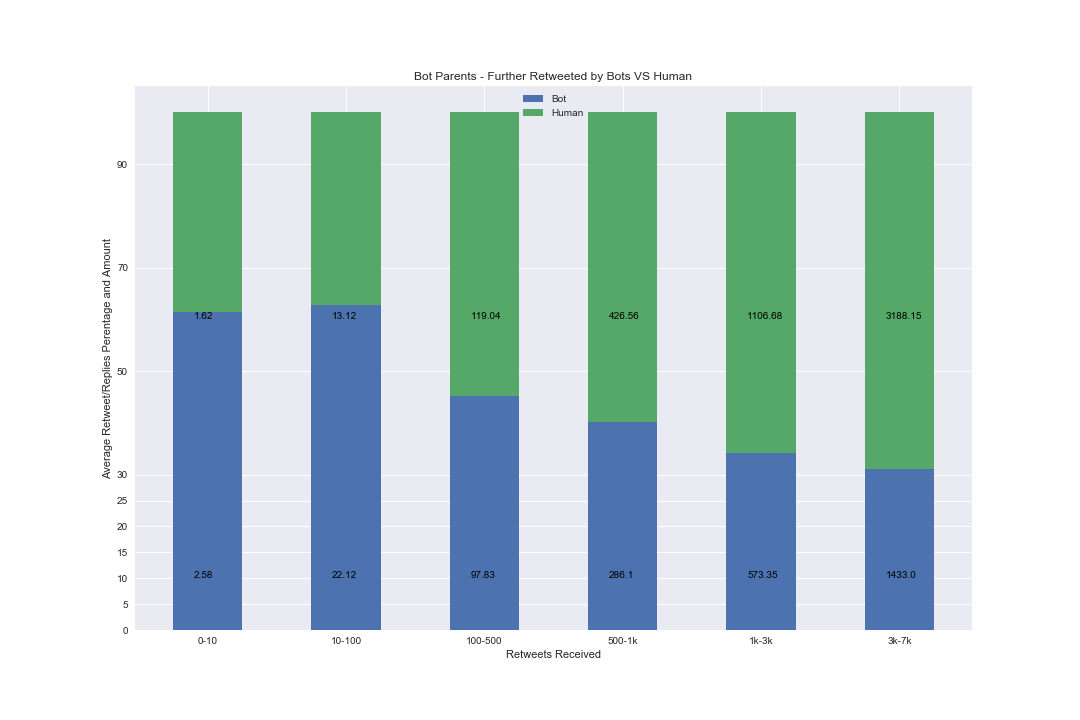
\includegraphics[width=\linewidth]{images/bots_furtherretweeted.png}
      \caption{Bots Parents}
      \label{fig:further_retweet_bots}
    \end{subfigure}
    \begin{subfigure}[b]{1\linewidth}
      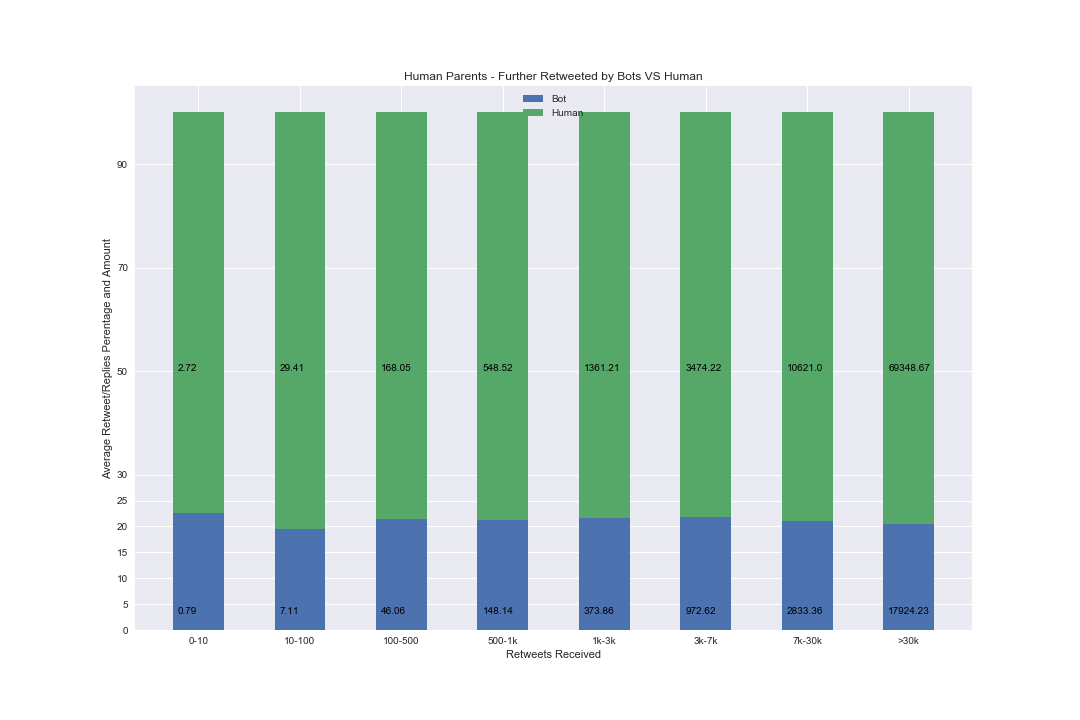
\includegraphics[width=\linewidth]{images/humans_furtherretweeted.png}
      \caption{Humans Parents}
      \label{fig:further_retweet_humans}
    \end{subfigure}
    \caption{Further Retweet}
    \label{fig:further_retweet}
\end{figure}

Next, we compared the cascades started by bots and humans. The cascades were grouped by their length to visualize the differences accurately. 
In Figure \ref{fig:further_retweet_bots}, we can see that the percentage of bots was high for smaller cascades started by bots. As the size of Cascade increases, the percentage of bots decreases. 
We made the opposite observation for humans in Figure \ref{fig:further_retweet_humans}. If a tweet receives few audience, they are most likely the followers. This means that bots are mostly
followed by bots and humans by humans. Thus, this finding goes in line with those made by earlier research which shows that bots and humans create a follower cluster dominated by their type.

To further analyze this, in Figure \ref{fig:humans_bots_percentage}, we look at the successful tweets and the early retweets. The early audience of a Tweet are the follower of the Original Poster (OP). If a Tweet becomes famous,
it goes beyond the followers. From the figure, we can see that the number of bots is high in first one percent of the retweets/replies for successful tweets in case of bots and is high for humans in a decreasing amount. This analysis provides further support to the assertion made in the previous paragraph.

\begin{figure}
    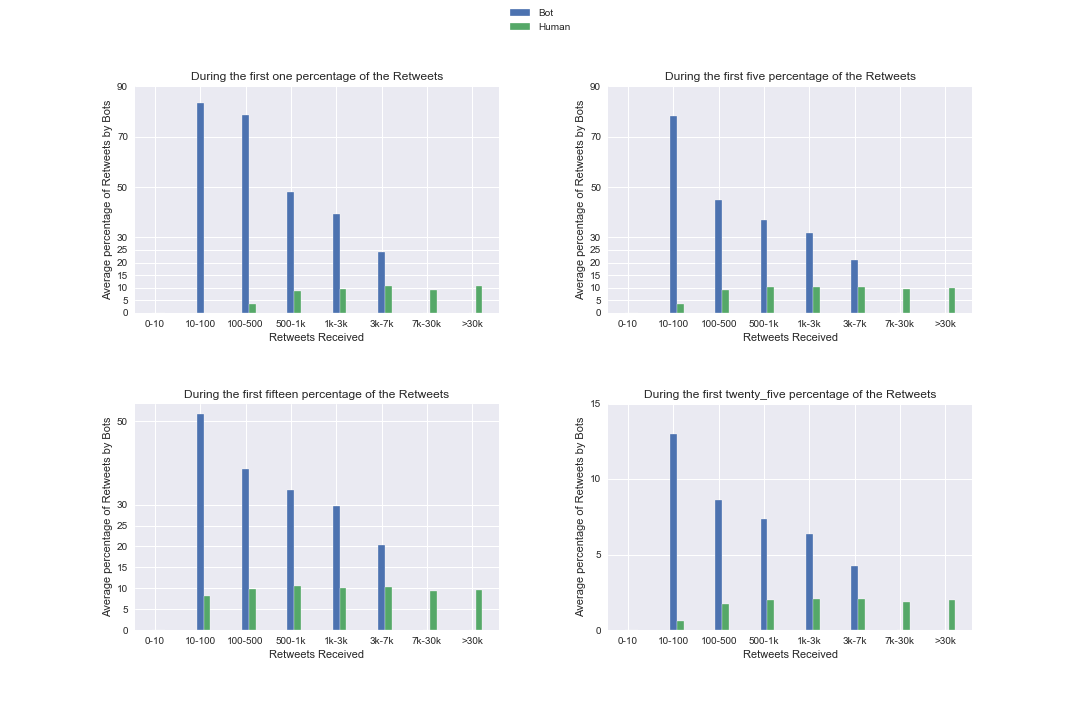
\includegraphics[width=\linewidth]{images/bot_humans_retweet_percentages.png}
    \caption{At Different Percentage Intervals}
    \label{fig:humans_bots_percentage}
\end{figure}



\subsection{Retweet Influence Analysis}

The average influence of a human was 4.06, half that of a bot, which was 8.12. This finding is similar to 
\cite{rizoiu2018debatenight}'s finding who found that bots were 2.5 times more influential than humans. Then influence for each user was converted 
into a percentage to determine how influential a user was. 

\begin{figure}[h!]
    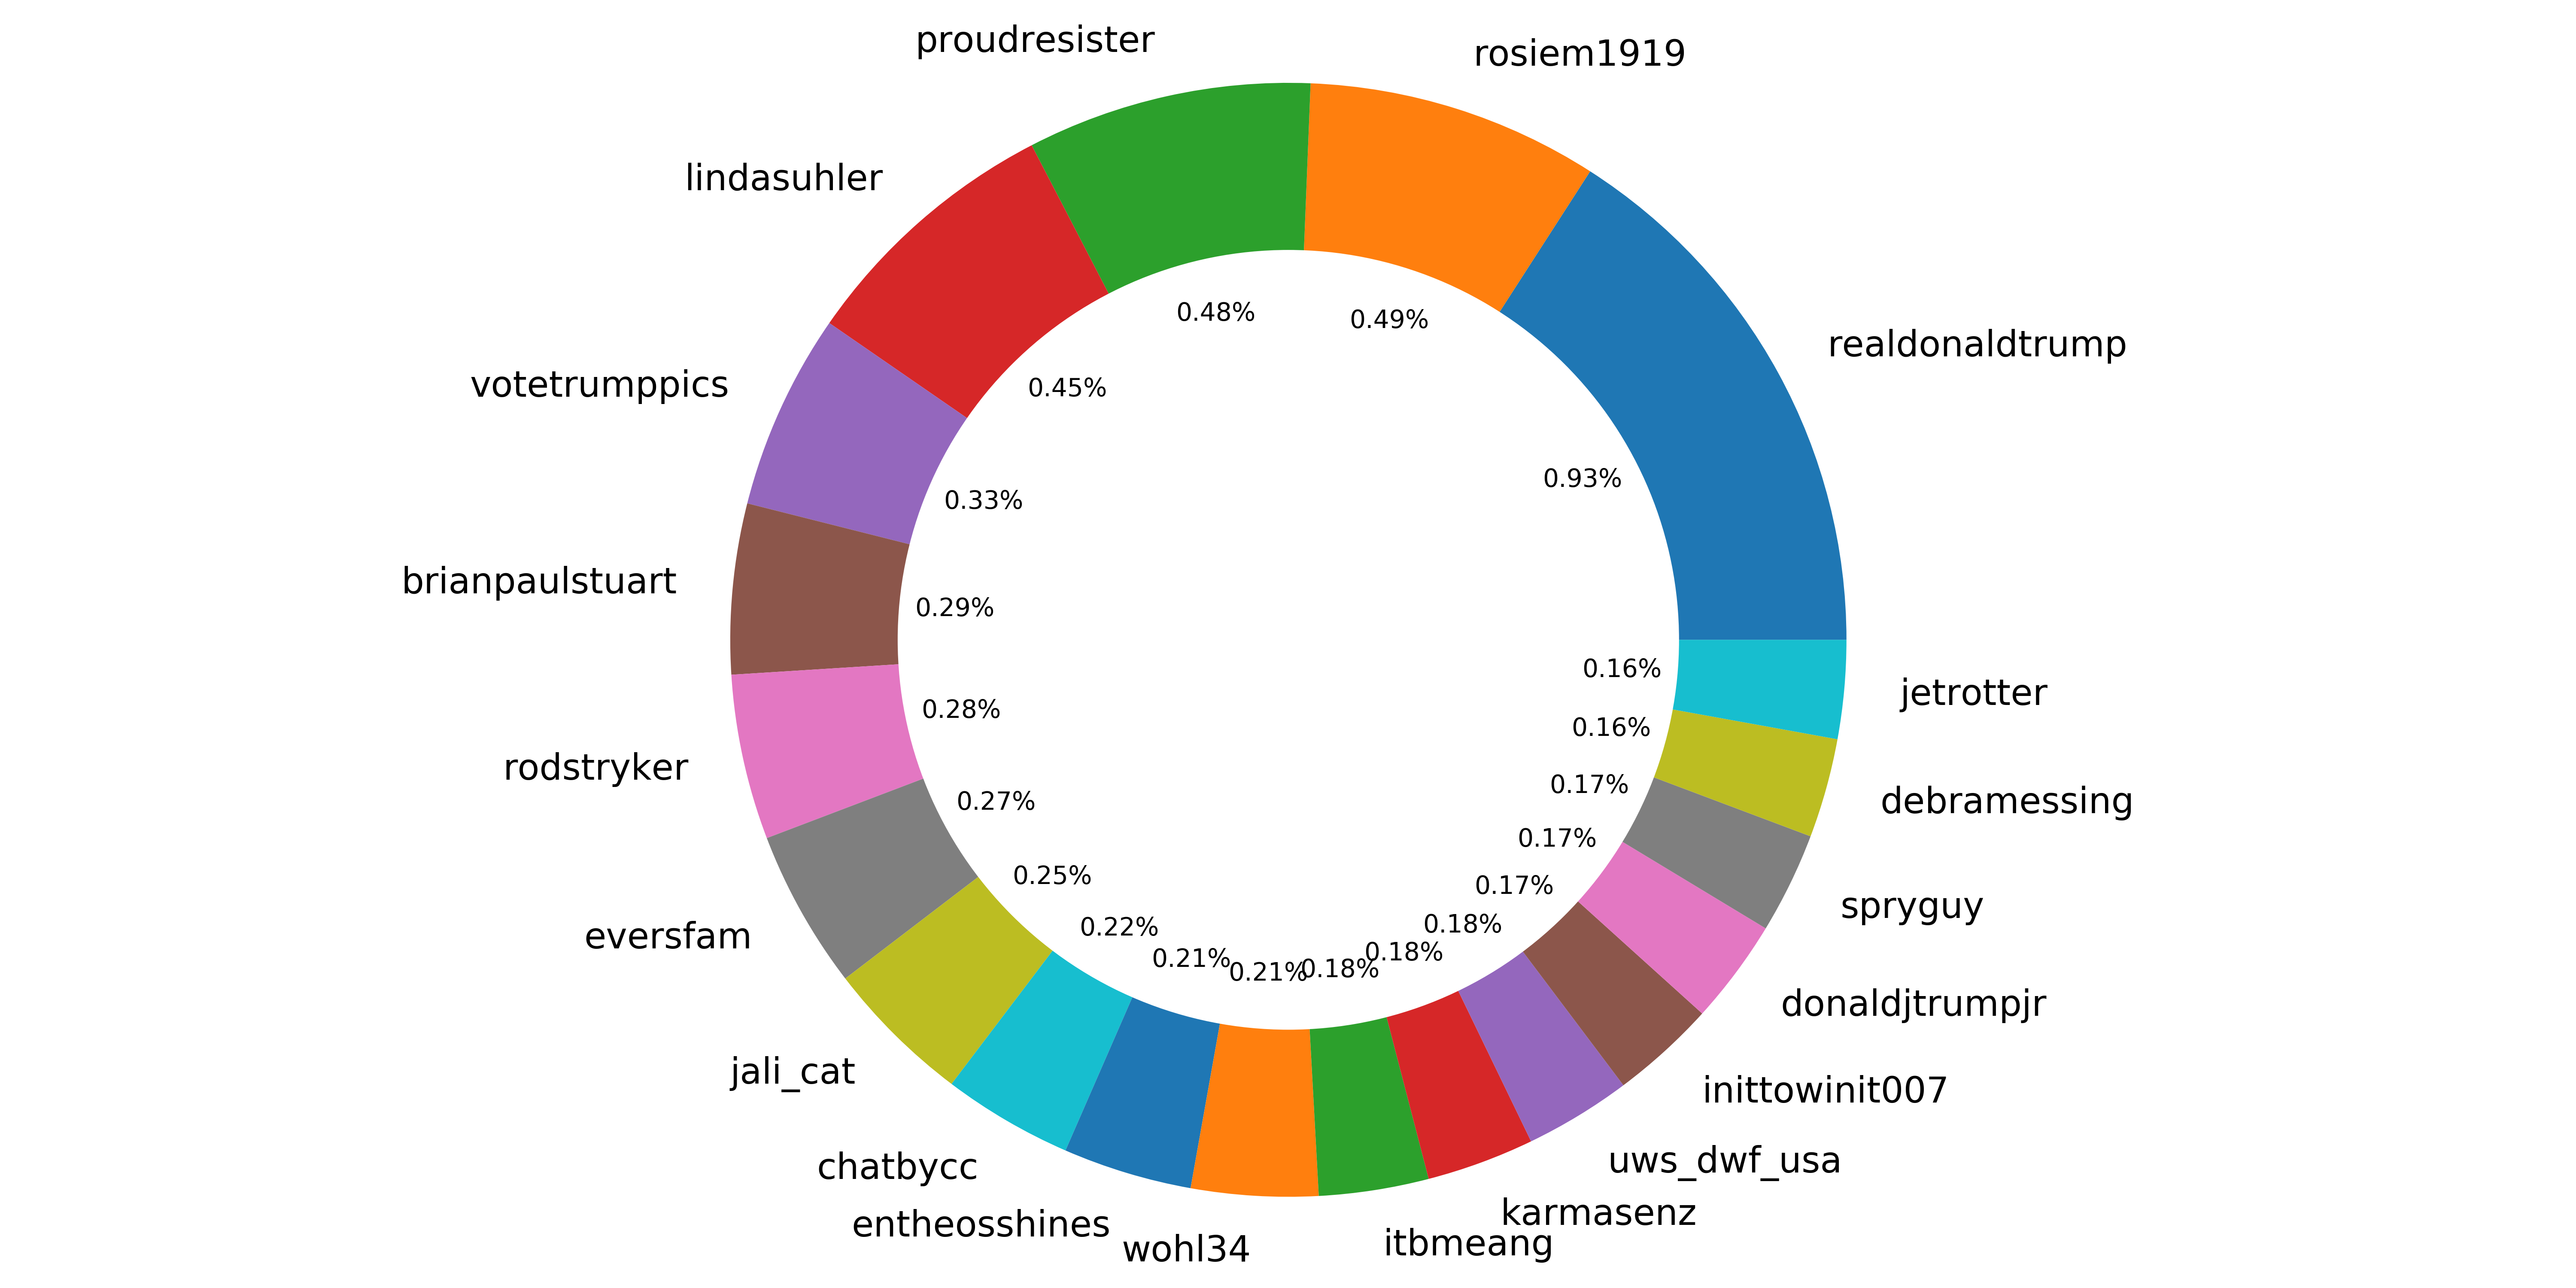
\includegraphics[width=\linewidth]{images/top_influences.png}
    \caption{Most influential users}
    \label{fig:humans_bots_percentage}
\end{figure}

Figure \ref{fig:humans_bots_percentage} unsurprisingly shows that the most influential user, who was possibly responsible for the creation of as much as 0.93\%
of the tweets was the POTUS, @realDonaldTrump.\par


\begin{figure}
    \centering
    \captionsetup{justification=centering}

    \begin{subfigure}[b]{0.4\linewidth}
      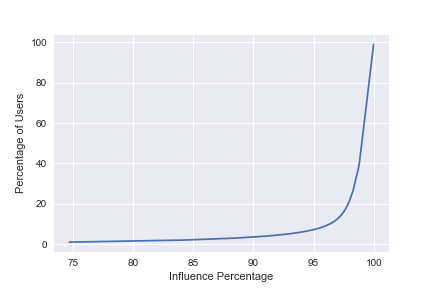
\includegraphics[width=\linewidth]{images/top_1per_bots.png}
      \caption{Bots}
    \end{subfigure}
    \begin{subfigure}[b]{0.4\linewidth}
      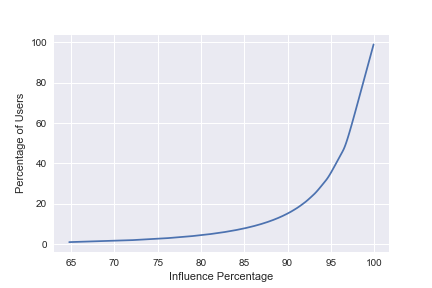
\includegraphics[width=\linewidth]{images/top_1per_humans.png}
      \caption{Humans}
    \end{subfigure}
    \begin{subfigure}[b]{0.8\linewidth}
        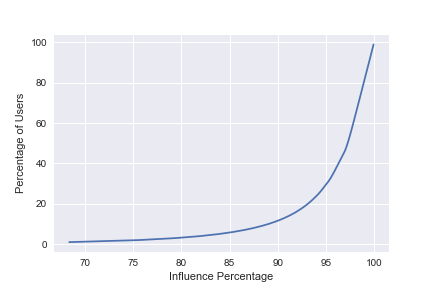
\includegraphics[width=\linewidth]{images/top_1per_all.png}
        \caption{All}
    \end{subfigure}
    \caption{Percentage of top users and their influence percentage}
    \label{fig:top_infuence}
\end{figure}

Then, we find the difference in influence made by the top 1\% of all users, top 1\% of the bots, and top 1\% of the Humans. To find this out, we first calculated the user wise 
influence of all users in our dataset as a sum of their influence in all their tweets. Then, we used our bot prediction to find bot user and bot influence. We calculated the Influence
 percentage by using the total influence of all users. Figure \ref{fig:top_infuence}, shows that 
the top 1\% of bots were responsible for 75\% of influence made by bots. Top 1\% of humans were responsible for 65\% of the influence. The top 20\% of bots are responsible for nearly 98\% of the influence. The top 20\% of humans are responsible for 64\% of total influence. \par

1\% of the bots are responsible for 11\% of the total influence. Out of 4.8M data in our cascade, this might imply that
bots were responsible for the creation of 500k human tweets. However, we cannot make this conclusion without further research. 
When calculating influence, we could have calculated the influence of a bot or a human in the diffusion graph multiple times. We use the graph in \ref{fig:diff_graph} to illustrate 
the problem in making this assumption.

\begin{figure}[h!]
    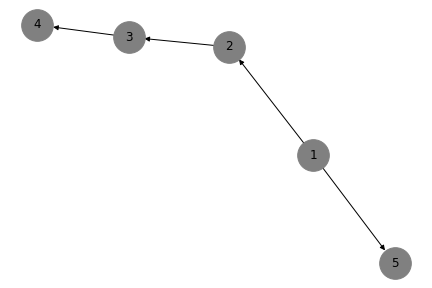
\includegraphics[width=\linewidth]{images/diffusion_graph.png}
    \caption{Diffusion Graph}
    \label{fig:diff_graph}
\end{figure}

In Figure \ref{fig:diff_graph} the influence score of node 1 will be 4, node 2 will be 2, of node 3 will be 1, and of node 4 and node 5 will be 0. If 1 and 2 are bots, 
the total bot influence score will be 6. However,1 created 
2. Although this disparity might cancel out in 2 large groups across a large dataset when taken in percentage, we still refrain from making that conclusion. 
Further research is needed to make 
this verification. If we can make the verification, we can measure the impact of bots in terms of monetary value by comparing it with the advertising cost.

\subsection{URL Influence Analysis}
Before performing URL influence calculation, we resolved short URLs and removed twitter.com links. We kept the URLs which we could not resolve as they were. 
652,054 unique URLs belonging to 157,192 unique domains were shared in our dataset by 652,054 unique users 1.9 Million times. Ten most popular domains in our dataset with their frequency are
in Table \ref{tab:Common_urls}. The top 10 domains for humans and bots, apart from t.co are in Table \ref{tab:common_human_bots}.

\begin{table}
    \centering
    \begin{tabular}{|l|l|}
    \hline
    \textbf{Domain Name} & \textbf{Frequency} \\ \hline
    t.co & 127717 \\ \hline
    vote.gop & 96127 \\ \hline
    thehill.com & 57476 \\ \hline
    cnn.com & 54129 \\ \hline
    youtube.com & 51347 \\ \hline
    wtxl.com & 38124 \\ \hline
    nytimes.com & 35863 \\ \hline
    foxnews.com & 35277 \\ \hline
    instagram.com & 31634 \\ \hline
    breitbart.com & 30290 \\ \hline
    pscp.tv & 27702 \\ \hline
    \end{tabular}
    \caption{Most Common URLs}
    \label{tab:Common_urls}
\end{table}


\begin{table}
    \centering
    \begin{tabular}{|l|l|}
    \hline
    \textbf{Human} & \textbf{Bots} \\ \hline
    vote.gop & vote.gop \\ \hline
    thehill.com & youtube.com \\ \hline
    cnn.com & foxnews.com \\ \hline
    youtube.com & breitbart.com \\ \hline
    wtxl.com & thegatewaypundit.com \\ \hline
    nytimes.com & pscp.tv \\ \hline
    foxnews.com & cnn.com \\ \hline
    instagram.com & instagram.com \\ \hline
    breitbart.com & thehill.com \\ \hline
    pscp.tv & facebook.com \\ \hline
    \end{tabular}
    \caption{Most Common Human and Bots URL}
    \label{tab:common_human_bots}
\end{table}

A single URL was shared 27.84 times in 1.97 cascades on average.
Next, we compare the average influence bots had on the URL cascades with the number of bots.

\begin{table}
    \centering
    \begin{tabular}{|l|l|l|l|l|}
    \hline
    Size & Amt & Influence \% & Average \% & \( \frac{Influence \%}{Average \%} \) \\ \hline
    0-10 & 98709 & 15.83 & 15.1 & 1.05 \\ \hline
    10-100 & 15309 & 19.67 & 14.84 & 1.33 \\ \hline
    100-500 & 1879 & 23.02 & 13.53 & 1.7 \\ \hline
    500-1k & 209 & 23.24 & 11.02 & 2.11 \\ \hline
    1k-3k & 122 & 21.53 & 9.23 & 2.33 \\ \hline
    3k-7k & 25 & 24.49 & 8.82 & 2.78 \\ \hline
    7k-40k & 5 & 14.92 & 7.77 & 1.92 \\ \hline
    \end{tabular}
    \caption{Percentage of Bots and their Influence}
    \label{tab:percentage_influence}
\end{table}

In Table \ref{tab:percentage_influence}, the size row denote the size of Cascade, Amount refers to the number of cascades of that size, Influence \% is the percentage of all influence 
made by bot users at that cascade group, and Average \% is the percentage amount of bots in that cascade group. We can observe that the ratio of influence to size is increasing as the 
size of cascade increases except for the last value. The difference in the last interval might be due to small sample size. 
This implies that over successful URL's, the impact of bot is higher.

\section{Conclusion, Limitations and Further Work}
In this study, we show that bots have been highly influential and that most of the influence comes from a few top bots. In line with previous research, we have also shown that bots 
and humans form a cluster around each other and join when a tweet gets successful. This knowledge can help to point out a possible direction in the fight against bots. 

\begin{itemize}
    \item We performed this study in a limited dataset. It would have been better to perform it in the complete data. However, we did not have access to it. 
    Twitter Firehose API or Search API can be used in the future to have complete access to the data. Apart from Firehose and Search API, 
    a mechanism for finding Twitter posts using Twitter's snowflake algorithm looks promising \cite{bettermetrics2019}
    \item The current analysis was done by considering all bots as a single entity. Although easy, this distinction has many flaws. In futures, attempts should be made to 
    divide different types of bots and study their agenda
    \item As Twitter attracts some demographics more than others, using random Twitter data is not representative of the nation or the voting population. 
    Careful clustering can be done to create a representative data to get representative influence in the future.
    \item The validation of the influence detection algorithm can be done in a better way. Even Machine Learning techniques can be used to make a better influence detection algorithm 
    to predict the diffusion edges.
    \item Reddit can be analyzed along with Twitter to create a better spread graph. A bot detection system can be made for Reddit too. Combining multiple sources, a
     long term study can be conducted to measure the success/failure of bots in changing people's opinion.
\end{itemize}

\bibliographystyle{aaai}
\bibliography{references}

\end{document}